\section{Scalogram interpretation}

The scalorgrams show the time frequency analysis content of the data for each region. Frequencies of higher magnitude will show up with brighter colors, which can also be seen on the magnitude colorbar for comparison of the magnitude with related values.
The frequency of the scalograms varies from 2.7370 Hz to 0.0031 Hz. This means according to the litterature, that bands of cardiac, respiratory, endothelial, myogenic and neurogenic is represented in the wavelet frequency span for the time frequency analysis. \cite{grayer2004}

The scalogram in \figref{fig:uncuffed_sub3_roi8_corr} is representing the wavelet transformation of the raw signal of region eight from subject three.

\begin{figure}[H]
	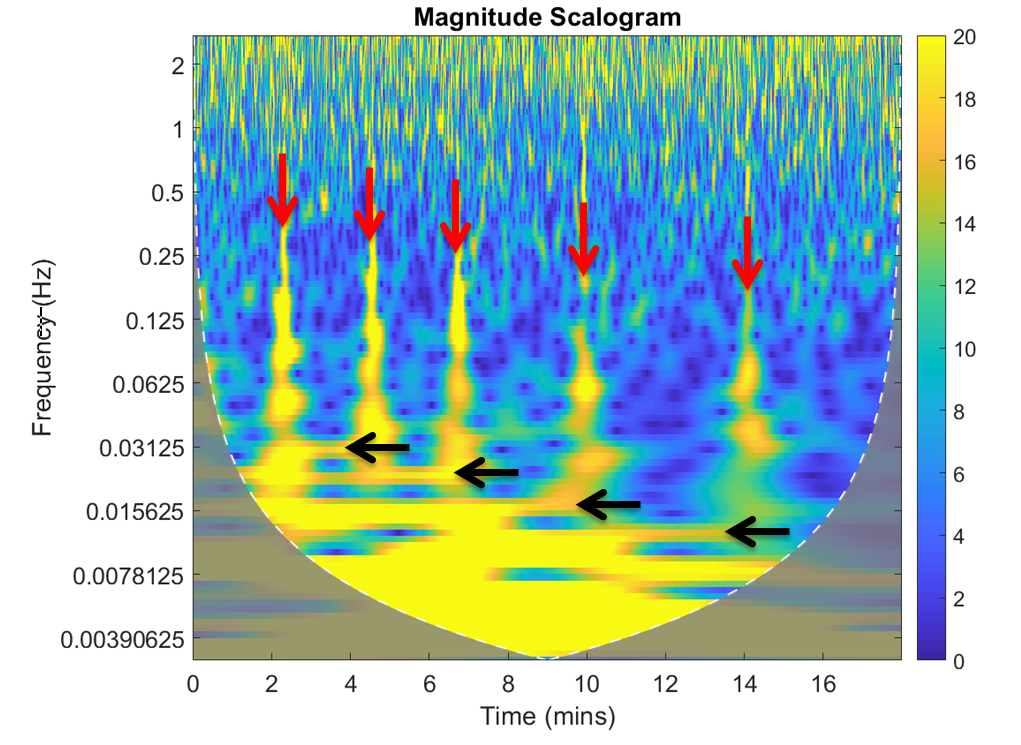
\includegraphics[width=0.7\textwidth]{figures/uncuffed_sub3_roi8_uncorr}
	\caption{Scalogram from the raw data of region eight in the uncuffed recording of subject 3, where high spike magnitudes can be seen induced by the jumps.}
	\label{fig:scalogram_uncorr}
\end{figure}

Looking at the scalogram from the raw signal in \figref{fig:scalogram_uncorr} the jumps can easily be seen as the hight spikes which represents the jumps in the signal. Five jumps is indicated with the red arrows are present in the scalogram at timepoints around 2.3, 4.4, 6.6, 10 and 14.1 in the 
signal from the scalogram. The jumps in the same signal shown in the time domain shows jumps at the same timepoints \figref{...} \fxnote{change the figure in the correction method so it fits to the scalogram? else we will have to show it in this section}. As stated in \ref{sec:artifacts} the jumps are induced by the shutter to make autocorrections for the array in the thermal camera because the temperatures are drifting. Different artifact components are represented in the signal. 

The artifact components of the raw signal can be sorted into three categories: 
\begin{itemize}
	\item White noise artifacts
    \item Drift between each interval
	\item Jumps
%	\item Generel drift in the signal
\end{itemize}

White noise artifacts is containing all frequencies and is therefore present in all if the experimental data why this can be looked past because this is constant for every subject. \fxnote{a reference is needed here}. The artifact components is disturbing the signal to make the cwt analysis valid because the artifacts is not constant in each recording.....
....
After the drift correction is added to the signal, the energy  has been reduced at this area induced from the jumps and drift. With this correction it should be more accurate to use the data for the statistics because. The signal should still be  preserved. 

\begin{figure}[H]
	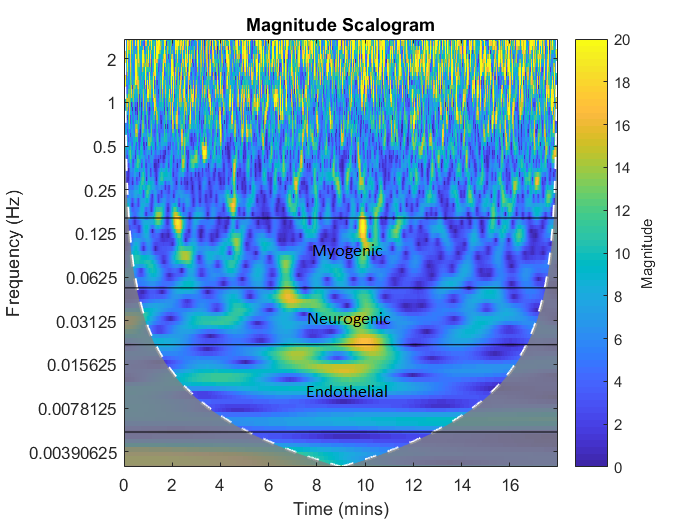
\includegraphics[width=0.7\textwidth]{figures/uncuffed_sub3_roi8_corr}
	\caption{Scalogram from the corrected data of region 8 in the uncuffed recording of subject 3, where a dampening of the spikes and  induced by the jumps has been achieved.}
	\label{fig:scalogram_corr}
\end{figure} 